%!TEX root = ../BGP_for_networks_who_peer.tex
\chapter{BGP Security}
\label{ch:security}
\section{Introduction}
BGP itself does not have much security mechanisms built in. You can secure your sessions with a \gls{MD5} hashed password, but that's about all.

That does not mean that your network's lifeline has to be insecure. There are methods you can use to protect yourself and also to protect the Internet from harm. This chapter shows these methods, and it is recommended that you at least implement some of them.

The \emph{robustness principle} as formulated by Jon Postel does not really apply to BGP announcements:
\begin{quote}
  ``Be conservative in what you send, be liberal in what you accept''
\end{quote}
(It does apply to the BGP protocol itself, though).

You must check and filter what others send you in terms of prefixes, and you must also be strict in what prefixes you send to others. Especially for the latter, it is often helpful to over-provision filters (like filter using communities and also filter out IPv4 networks smaller then /24).

\rfc{7454} is the reference document for BGP routing security. This chapter will heavily quote from it. Please read the original for further reference.

\section{Automation}
A lot of the measures explained here work on rules and data that might change over time. So it is a good idea to build some automation:
\begin{itemize}
  \item Automate updating rules on all of your routers at once
  \item Automate checking rules and then update your implementation of these rules.
\end{itemize}
What you use for automation is up to you - it depends on your IT and network management environment.

\section{Simple measures}
\subsection{Maximum prefixes}
\label{maxprefix}
This parameter is configured for each eBGP session and is the simplest and easiest security measure you can use. Unfortunately, many stop here. Please do not.

Maximum prefix defines a limit for the number of prefixes you accept from an eBGP peer. If the peer sends more, the eBGP session is shut down. Usually, routers keep the session down for some time, then it is automatically re-enabled. If the peer still sends more prefixes than allowed, it is shut down again.

For selecting this limit, the following rules of thumb can be used:
\begin{itemize}
  \item For sessions to \emph{peers}, the limit should be less than the total number of prefixes in the Internet. Set it at least to ten times the normal number of prefixes your peer announces. This protects you against your peer announcing the full routing table to you, but still allows normal growth. Check and adjust from time to time (or even better: Automate this).
  \item For sessions to your \emph{upstream} provider, you must, of course, set the limit higher than the total number of prefixes in the Internet. It must be high enough to accommodate normal growth, so either set it \emph{very} high or check and adjust it regularly. Otherwise, there can be surprising session shutdowns. This protects you against gross misconfigurations at your upstream provider (like sending you a lot of de-aggregated prefixes).
\end{itemize}

\subsubsection{Maximum prefixes for announcements}
Some BGP implementations (notably \emph{FRRouting}) have implemented a maximum prefix parameter for announcements: This protects your peers from you accidentally flooding. Simply set it to the number of prefixes you normally announce, add some leeway for growth, and use automation to keep track of the value you set.

In case you make a mistake with your filtering this guarantees to not send more than the configured number of prefixes. However, \emph{which} prefixes you send you cannot influence, this limits the usefulness of this feature.

Example for FRRouting:
\begin{verbatim}
  router bgp 64500
  ...
  neighbor 10.96.1.1 maximum-prefix-out 85
\end{verbatim}
This allows you to announce up to 85 prefixes to your neighbor.

\section{Protecting your router}
A complete discussion about how to protect a router is outside the scope of this document; here we will focus on BGP and how to protect yourself.

BGP itself has some protection mechanisms - BGP packets from IP addresses not configured are discarded. However, in some routers, this happens in the control-plane and consumes CPU cycles. A possible attack vector could exploit this by simply trying to overload your CPU. A countermeasure can be to use an explicit filter to disallow everything to port 179 from sources which could never be a BGP peer.

\section{Protecting your BGP sessions}
\subsection{Motivation}
The idea of these measures is to protect your TCP-based BGP sessions against attacks. Keep in mind, these TCP sessions are long-living (speaking of weeks and months), so an attacker can take its time to try to destroy a BGP session by sending crafted packets.

\subsection{MD5 session password}

The easiest countermeasure against TCP based attacks on BGP sessions is to use an \gls{MD5} protection as described in \rfc{2385}. When implementing this, keep in mind to also implement some key (password) handling procedures (just imagine your router has to be replaced and you have to re-create all eBGP configurations).

Example for setting an MD5 password on Cisco:
\begin{verbatim}
  router bgp 64500
  ...
  neighbor 10.96.1.1 password mysecretpassword
\end{verbatim}

Example for Mikrotik:
\begin{verbatim}
  add name=AS64496 remote-as=64496 \
    remote-address=10.96.1.1 tcp-md5-key=mysecretpassword
\end{verbatim}

\subsection{TCP Authentication Option}
\gls{MD5} which is widely used is considered to be insecure and deprecated. To replace it \rfc{5925} defines a mechanism called \emph{TCP Authentication Option}, please read the RFC for details. In short, it uses stronger codes to protect your session.

\subsection{TTL security}
Instead, relying on the \gls{TTL} value of incoming TCP packets is easier to handle and to implement. \rfc{5082} describes how setting the TTL value of packets when sending to 255, and checking that value when receiving, makes it an impossible-to-spoof security measure. As the TTL is decreased by every hop, when you receive a packet with TTL 255, it \emph{must} have been sent by a directly adjacent node.

This feature must be set on both ends to work - if you set it on one end only, one side sends IP packets with a \gls{TTL} of 1, and the other with a \gls{TTL} of 255, and a session cannot be established.


On Cisco, you configure TTL security such as
\begin{verbatim}
  router bgp 64500
  ...
  neighbor 10.96.1.1 ttl-security hops 1
\end{verbatim}

On Mikrotik, you do not configure how many maximum hops a peer can be away, but the TTL value, which is 255 for directly adjacent peers (this is also the default value):
\begin{verbatim}
  add in-filter=upstream-in name=AS64496 out-filter=upstream-out \
    remote-address=10.96.1.1 remote-as=64496 ttl=255
\end{verbatim}

\section{BGP filtering}
A ``raw'' BGP full feed (the so-called ``global routing table'') contains a lot of junk you do not want in your routers. In the best case, it contains prefixes to non-routable networks; in the worst case, it can break your internal routing.

There are a number of measures to filter a full BGP feed which will be explained in the following sections.

In general, we have three sources of information to fill your BGP table:
\begin{itemize}
  \item the raw input you receive from your peers
  \item one or more \emph{block lists} where you define what you not want from that specific peer or from all peers
  \item an \emph{allow list} or whitelist, where you define what you allow from that peer
\end{itemize}

Job Snijders defined that in \cite{ripe77jsbgp} as intersecting sets, see
Figure~\ref{fig:goodbadugly}.

\begin{figure}
  \centering
  \includegraphics[width=\linewidth,page=14]{img/Drawings.pdf}
  \caption{BGP prefix lists as intersecting sets according to \cite{ripe77jsbgp}}
  \label{fig:goodbadugly}
\end{figure}

\section{Inbound: Prefix filtering}
\label{sec:inboundprefixfiltering}
Prefix filters work on received prefixes only. Some of them are easy to implement, while some require more effort. Sometimes the shortest solution to implement is not the best, it often is better to have more lines of config to increase readability.

When implementing, it's helpful to write down your rules in pseudo-code to find out the best order of statements.

\subsection{Filtering against prefix sizes}
Normally (there are exceptions), prefixes are announced in certain minimum and maximum sizes in the global Internet routing table. Currently, they are:
\begin{description}
  \item[IPv4, minimum size] is /24. No smaller networks should be announced. Possible exceptions: \Gls{blackholing}, or an announcement in combination with a NO-EXPORT community set from customers.
  \item[IPv6, minimum size] is /48. Same exceptions as within IPv4.
  \item[IPv4, maximum size] is a /8. Larger networks are not announced. Depending on your set-up, you might want to accept the \gls{default-route} 0.0.0.0/0 from one of your upstreams.
  \item[IPv6, maximum size] is currently a /16 (please take this with a grain of salt, this number might already have changed). The remark about accepting a \gls{default-route} ::0 is the same.
\end{description}

\subsubsection{Implementation example: Cisco}
As often, there is more than one way to implement this:
\begin{verbatim}
  ip prefix-list ipv4-small-networks permit 0.0.0.0/0 ge 25 le 32
  ip prefix-list ipv4-large-networks permit 0.0.0.0/0 ge 1 le 7
  !
  route-map upstream-in deny 50
    match ip address prefix-list ipv4-small-networks
  !
  route-map upstream-in deny 55
    match ip address prefix-list ipv4-large-networks
\end{verbatim}
Explanation:
\begin{itemize}
  \item We first define two prefix-lists, matching all prefixes (``0.0.0.0/0'' here means all prefixes, not the default route) with a length greater or equal to 25 ``ge 25'' and less or equal to 32 ``le 32'' (the ``le 32'' is not really necessary and may be removed by the router's command parser).
  \item We do the same for too large networks (from length 1 to 7).
  \item We then insert a deny-rule into our upstream-in route-map with the prefix-lists we defined as match-part. Deny-rule means that when a prefix matches all match-statements, the whole route-map terminates and the prefix is \emph{not} let through.
\end{itemize}

Alternative (shorter, more elegant) implementation with just one prefix-list:
\begin{verbatim}
  ip prefix-list ipv4-unwanted permit 0.0.0.0/0 ge 25 le 32
  ip prefix-list ipv4-unwanted permit 0.0.0.0/0 ge 1 le 7
  !
  route-map upstream-in deny 50
    match ip address prefix-list ipv4-unwanted
\end{verbatim}
This has the additional advantage that you can add even more prefixes to it that you not want (see below). This shortens your configuration but might also decrease readability.

And for IPv6:
\begin{verbatim}
  ipv6 prefix-list ipv6-unwanted permit ::/0 ge 49 le 128
  ipv6 prefix-list ipv6-unwanted permit ::/0 ge 0 le 18
  !
  route-map upstream-in deny 45
    match ipv6 address prefix-list ipv6-unwanted
\end{verbatim}

\subsubsection{Implementation example: Mikrotik}
Mikrotik works with filter-lists instead of route maps, but for easier readability you can use sub-filters:
\begin{verbatim}
  /routing filter
  add action=jump chain=upstream-in jump-target=ipv4-size
  ...
  add action=reject chain=ipv4-size prefix-length=0-7
  add action=reject chain=ipv4-size prefix-length=25-32
\end{verbatim}

\subsection{Filtering against RPKI-Invalid prefixes}
\gls{RPKI} allows the holder of a resource (an IPv4/IPv6 prefix) to cryptographically prove that it is really the holder and allows via defining \glspl{roa} how that prefix can be announced via BGP.

RPKI is defined in \rfc{6480}, ROAs are defined in \rfc{6482}. For more information about RPKI see \url{https://rpki.readthedocs.io/}.

A \gls{roa} is a triple containing the following values:
\begin{itemize}
  \item The prefix itself (network plus prefix length)
  \item An \gls{AS} which is allowed to originated that prefix
  \item A maximum prefix length for which BGP announcements are allowed, this can be the same as the prefix length of the network (in this case the announcement of more specifics for this prefix is not allowed).
\end{itemize}

 To use RPKI and ROAs you need a host running a \gls{RPKI validator}. This validator fetches resource certificates and \glspl{ROA} from \glspl{RIR}, checks their signatures and is then available being contacted by routers using RPKI-RTR protocol (defined in \rfc{8210}). You can (and should) have more than one validator.

 Routers simply receive a list of validated prefixes, their allowed originating AS number and a range of allowed networks masks. This can be used to check prefixes received via eBGP. Result of this check is one of three possible values:
 \begin{description}
   \item[Valid:] A \gls{ROA} for this prefix exists, the originating AS matches and the announced prefix length is covered.
   \item[Invalid:] A ROA for this prefix exists, but either it is for a different originating AS number or the prefix length is \emph{not} covered (too specific).
   \item[Unknown:] For this prefix a ROA does not exist. This result is also returned if no validator is reachable by the router.
 \end{description}

Recommendation for your filtering rules:
\begin{itemize}
  \item \emph{Accept} prefixes with \emph{valid} or \emph{unknown} result.
  \item \emph{Deny} prefixes with result \emph{invalid}.
\end{itemize}

\subsubsection{Implementation example: FRRouting}
You have to use a route-map to filter out \emph{RPKI invalid} prefixes (only relevant config statements are shown):
\begin{verbatim}
rpki
  rpki cache a.b.c.d 3323 preference 1
  exit
!
router bgp 64500
 neighbor upstream peer-group
 neighbor upstream-v6 peer-group
 address-family ipv4 unicast
  neighbor upstream route-map upstream-in in
 exit-address-family
 address-family ipv6 unicast
  neighbor upstream-v6 route-map upstream-v6-in in
 exit-address-family
!
route-map upstream-in deny 50
  match rpki invalid
!
route-map upstream-v6-in deny 50
  match rpki invalid
\end{verbatim}

\subsubsection{Cisco}
When RPKI is active and a connection to a validator is established, Cisco filters out \emph{invalids} by default. To prevent this, you have to either disable it completely or allow invalid announcements to become ``best'' explicitly (see commented out commands below):

\begin{verbatim}
router bgp 64500
  bgp rpki server tcp a.b.c.d port 3323 refresh 300
  address-family IPv4
   ! bgp bestpath prefix-validate allow-invalid
   ! bgp bestpath prefix-validate disable
  exit-address-family
  address-family IPv6
   ! bgp bgp bestpath prefix-validate allow-invalid
   ! bgp bestpath prefix-validate disable
  exit-address-family
\end{verbatim}

Route-map statements are the same as for FRRouting - but you only need them if you have ``\emph{bgp bestpath prefix-validate allow-invalid}'' configured.


\subsection{Filtering against non-routable prefixes}
When IPv4 was created, the inventors reserved certain part of the address space for specific purposes. These were the times of class-A,B,C networks (if anybody still mentions them - the concept was abolished in 1993 in some RFCs starting with \rfc{1517}).

The following IPv4 space is still considered to be not routable and should never be announced via BGP:
\begin{description}
  \item[Private IPv4 space] as defined in \rfc{1918}. Networks \emph{10.0.0.0/8}, \emph{172.16.0.0/12} and \emph{192.168.0.0/16} are reserved for private use and should never be announced.
  \item[IPv4 networks reserved for documentation purposes] defined in \rfc{5737}. These three networks are reserved and should not be routed (but you might see them in this document as example networks).
  \item[Reserved for multicast:] The address block \emph{224.0.0.0/4} was reserved for multicast and cannot be used for anything else. Do not accept announcements out of it via BGP.
  \item[So-called ``Class-E'':] The network block \emph{240.0.0.0/4} was always reserved ``for future use'' which never came. Today this range is considered to be not usable and therefore should not be accepted via BGP.
  \item[More can be found] at this IANA website: \url{https://www.iana.org/assignments/iana-ipv4-special-registry/iana-ipv4-special-registry.xhtml}. Everything with ``Globally Reachable False'' should be filtered out.
\end{description}

In IPv6, there is a similar list at IANA \url{http://www.iana.org/assignments/ipv6-address-space}. However, for IPv6 it is easier to positive-filter for \emph{2000::/3}, as this is the only block where unicast address assignments were made from. Currently. You might check frequently if other blocks have been added. It is strongly recommended that you automate this task.

\subsubsection{Implementation example: Cisco}
For IPv4, you can simply add all unwanted prefixes to the list we defined in the previous section:
\begin{verbatim}
  ip prefix-list ipv4-unwanted permit 192.168.0.0/16 le 32
  ip prefix-list ipv4-unwanted permit 172.16.0.0/12 le 32
  ip prefix-list ipv4-unwanted permit 10.0.0.0/8 le 32
  ...
\end{verbatim}

\subsubsection{Implementation example: Mikrotik}
You can add this to your existing filter or you can create a sub-filter for better readability:
\begin{verbatim}
  /routing filter
  add action=reject chain=ipv4-unwanted prefix=192.168.0.0/16 prefix-length=16-32
  add action=reject chain=ipv4-unwanted prefix=172.16.0.0/12 prefix-length=12-32
  add action=reject chain=ipv4-unwanted prefix=10.0.0.0/8 prefix-length=8-32
  ...
\end{verbatim}

\subsection{More unwanted prefixes}
In the last section, we covered non-routable prefixes. But these are not the only ones you want to block.

\subsubsection{IXP LAN Prefixes}
When you are connected to an Internet Exchange Point, you have an interface configured with an IP address and netmask of that IXP. If, now, someone else announces the same network (or worse: a more specific sub-network) via BGP and you accept this announcement, your router might prefer this announcement over the one of its own interface (especially if the announcement \emph{is} more specific).

So it is strongly recommended that you  block BGP announcements of all IXP LANs you are connected to.

For DE-CIX Frankfurt, a filter for Cisco would look like:
\begin{verbatim}
  ip prefix-list ipv4-unwanted permit 80.81.192.0/21 le 32
  ipv6 prefix-list ipv6-unwanted permit 2001:7f8::/64 le 128
\end{verbatim}

For Mikrotik:
\begin{verbatim}
  /routing filter
  add action=reject chain=ipv4-unwanted prefix=80.81.192.0/21 prefix-length=21-32
  add action=reject chain=ipv6-unwanted prefix=2001:7f8::/64 prefix-length=64-128
\end{verbatim}

\subsubsection{Your own prefixes}
You also should protect yourself against hijacking of your own prefixes and against accepting announcement of your customers' prefixes.

Just imagine you accept an announcement of a more-specific subnet of the network you are using for your office\ldots or for your routers!

Commands to protect against this are the same - simply add your prefixes to the \emph{unwanted} lists you have already defined.

\subsubsection{Your customers' prefixes}
If your customers are single-homed to you, you should use the same measures as with your own prefixes.

In case your customers are multi-homed however, you should accept their prefixes, but perhaps not more-specifics of their prefixes.

\section{Route flap dampening}
\subsection{Motivation and history}
BGP is a protocol using incremental updates. Routes are announced and withdrawn if they are no longer valid. If this announce - withdraw happens too fast for prefixes we speak about \emph{flapping} routes. This consumes CPU cycles on all BGP speaking routers as each time a prefix flaps the BGP table (and also the routing table) needs to be updated.

So in 1998 \rfc{2439} was published to introduce \emph{route flap dampening} - which means that routes which flap too often are suppressed and only re-used once they become stable again. The original values for this dampening have been proven too aggressive, so in 2006 in \cite{ripe378} it was recommended to disable dampening completely.

\subsection{How does it work?}
Dampening works by increasing a penalty value each time a route flaps, which is then decreased over time. Once a configurable threshold has been reached, the route is suppressed. If over time the penalty is lower then another (lower) threshold, the route is no longer suppressed and re-used.


\subsection{Current recommendation}
More recent studies show that by adjusting the dampening parameters to be less aggressive route flap dampening can be made useful again. The documents \rfc{7196} and \cite{ripe580} give recommendations:
\begin{itemize}
  \item The ``penalty'' when starting suppression should be between 6000 (more aggressive) and 12000 (less aggressive). Default on most routers is 2000 (way too aggressive).
  \item To avoid ``surprises'' for operators, the default should not be changed.
\end{itemize}

\subsubsection{Configuration examples}
On Cisco you turn on flap dampening for each address family separately and you use a route-map to adjust parameters:
\begin{verbatim}
  router bgp 64501
    address-family ipv4
      bgp dampening route-map set-dampening-parameters
    exit-address-family
    address-family ipv6
      bgp dampening route-map set-dampening-parameters
    exit-address-family
  !
  route-map set-dampening-parameters permit 100
    set dampening 15 750 6000 60
  !
\end{verbatim}
Parameters set in the route-map are explained below.

FRRouting is similar, except you do not need a route-map to set the parameters (this has the slight disadvantage that you cannot tune dampening individually through match statements in the route-map). Also in the current release of FRRouting BGP dampening is only working for IPv4 unicast and multicast:
\begin{verbatim}
  router bgp 64501
    address-family ipv4 unicast
      bgp dampening 15 750 6000 60
    exit-address-family
\end{verbatim}

\subsubsection{Parameters}
Both Cisco and FRRouting allow you to set the following parameters:
\begin{verbatim}
  ... dampening <half-life> <reuse-threshold> <suppress-threshold> <max-suppress>
\end{verbatim}

To understand them, you need to know that a \emph{penalty} is calculated for each route. The penalty is increased every time a route flaps.

These are the configurable parameters for the Cisco and FRRouting implementation:
\begin{description}
  \item[<half-life>] is the time value in minutes in which the penalty is reduced by half.
  \item[<reuse-threshold>] if the penalty gets lower than this value, the route becomes valid (unsuppressed) again.
  \item[<suppress-threshold>] if the penalty is higher than this, the route is started being suppressed.
  \item[<max-suppress>] is the maximum time (in minutes) a stable (non-flapping) route stays suppressed.
\end{description}

The following parameters are calculated:
\begin{description}
  \item[<max-suppress-penalty>] calculated value:
   \( <reuse-limit> * 2^{<max-suppress> / <half-life>}  \)
\end{description}

When setting the parameters you have to keep in mind:
\begin{itemize}
  \item \emph{<max-suppress-penalty>} must be larger than \emph{<suppress-threshold>}, otherwise a route never gets suppressed.
  \item the shorter you choose \emph{<half-life>} the faster a route gets unsuppressed.
  \item Cisco has a \emph{<maximum-allowed-penalty>} of 20000, your \emph{<max-suppress-penalty>} must be kept lower than this.
  \item choose \emph{<supress-threshold>} large enough that a small number of  flaps are still allowed, otherwise you risk that too many parts of the Internet become unreachable for you.
  \item \rfc{7196} gives recommendations how to set these values.
  \item Cisco simply turns off BGP dampening if you enter invalid values in the route-map (it gives a warning in the logging).
\end{itemize}

This paper explicitly gives no recommendation on how to set these values. Please read the RFCs and make your own decision depending on your operational needs.

\section{Inbound: Next-hop filtering}
When peering on an IXP LAN, your BGP peers can send you any IP address of this LAN as a next hop (not only their own). This is ok when peering with a route server (who does that as part of its functionality), but a ``standard'' peer should only send its own IP address as next hop (there might be an exception when a special address is used for signaling \gls{blackholing}).

So you can set the following in your route-map for direct peers (in this example you peer with AS64496 on 80.81.192.22 and with AS64497 on 80.81.192.43)
\begin{verbatim}
  ip as-path access-list 1 permit ^64496_
  ip as-path access-list 1 permit ^64497_
  !
  access-list 1 permit 80.81.192.22
  access-list 2 permit 80.81.192.43
  !
  route-map direct-peer-in permit 10
    match ip as-path 1
    match ip next-hop 1
    continue 500
  !
  route-map direct-peer-in permit 20
    match ip as-path 2
    match ip next-hop 2
    continue 500
  !
  route-map direct-peer-in deny 100
  !
  route-map direct-peer-in permit 500
  ! rest of processing starts here
\end{verbatim}
AS-Path and next-hop IP both have to match; if they do, the route-map jumps to entry 500 for further processing. If none of the route-map entries 10 or 20 matches, entry 100 stops processing with a ``deny'' result.  In this way you can have one route-map for all direct peers. Of course, you can also use a separate route-map for each peer.


\section{Inbound: AS-Path based filtering}
Even if a prefix is completely legit, it is still advisable to also check the AS path.

\subsection{Private AS numbers}
Like prefixes, there are AS numbers reserved which should never be seen in the global routing table.

So-called private ASes are like private IP addresses; they may be used within a provider's network, but should never be seen in the global routing table. They are defined in \rfc{6996}:
\begin{itemize}
  \item 16-Bit ASes: 64512 - 65534
  \item 32-Bit ASes: 4200000000 - 4294967294
\end{itemize}

\subsection{Special AS numbers}
Also, some AS numbers are set aside for documentation purposes.
\rfc{5398} lists them:
\begin{itemize}
  \item 16-Bit ASes: 64496 - 64511
  \item 32-Bit ASes: 65536 - 65551
\end{itemize}

At IANA, you can check which other AS numbers are reserved; they also should not be in an AS path: \url{https://www.iana.org/assignments/as-numbers/as-numbers.xhtml}

\subsection{Implementation example: Cisco}
Cisco supports regular expressions for parsing AS paths; in this case (filtering against unwanted ASes in a path) this is not really helpful. You need to build a regular expression list so that all unwanted ASes are matched:
\begin{verbatim}
  ! match 64496 - 131071
  ! match 64496 - 64499
  ip as-path access-list 100 permit _6449[6-9]_
  ! match 64500 - 64999
  ip as-path access-list 100 permit _64[5-9][0-9][0-9]_
  ! match 65000 - 69999
  ip as-path access-list 100 permit _6[5-9][0-9][0-9][0-9]_
  ...
  route-map upstream-in deny 40
    match as-path 100
\end{verbatim}
Numerical ranges would be more helpful here, but we can only use what router vendors implement.

When building regular expressions for filtering, keep in mind that your co-workers also need to understand them. Most of the time, it's better to add more lines to your filter list and keep your regular expressions simple.

\subsection{Inbound from customers: AS filtering}
ISPs should only accept prefixes from customers where every AS in the path either belongs directly to that customer or to a sub-customer. To scale this, use automation. This protects you and the whole Internet community from your customers' hijacking prefixes which do not belong to them (by faking an AS path).

\section{Inbound and outbound: BGP community handling}
We covered BGP communities in chapter~\ref{ch:BGP Communities}. A lot of Autonomous Systems use them. And attach them to prefixes. Which means that the prefixes you receive via eBGP might have a lot of (mostly) useless communities attached to them. However, even if they are useless to you, your transit customers might need or want them.

So it is recommended that you leave any BGP communities untouched, \emph{except} if they have your AS number in the high order part (this applies to all types of BGP communities: original, extended, and large).

You should only allow BGP Communities with your AS number in them in via eBGP:
\begin{itemize}
  \item If you allow customers (or peers) to use them to send you commands and
  \item on BGP connections to customers (or peers)
\end{itemize}

All other BGP communities with your AS in them should be removed inbound.

Outbound, you should only send out what you have documented so your customers or peers (or anybody else receiving your prefixes) can make use of it.  y
You should especially remove any communities you have set which have a private AS number in the higher part.

\section{Outbound: Sending prefixes}
The best way of not polluting the global routing table with bad prefixes would be if every provider behaved according to some code of conduct.

This is the goal of the MANRS initiative - MANRS stands for Mutually Agreed Norms for Routing Security. This is a set of rules an ISP (or IXP) can sign and so express its intent to keep the routing table (and the Internet) clean.

Details can be found at \url{manrs.org}, but basically to be compliant you need to agree to:
\begin{itemize}
  \item Prevent propagation of incorrect routing information.
  \item Prevent traffic with spoofed source IP addresses (outside of the scope of this paper).
  \item Facilitate global operational communication and coordination between network operators (= ``talk to each other and listen when someone talks to you'').
  \item Facilitate validation of routing information on a global scale (we covered this in \ref{sec:inboundprefixfiltering}).
\end{itemize}

\subsection{Prevent propagation of incorrect routing information}
The first step in not propagating incorrect prefixes via BGP is not to accept them. What is not in your prefix table cannot be propagated. So the measures described in \ref{sec:inboundprefixfiltering} should be applied.

Also, you can apply the same filter rules you already configured for incoming prefixes also in outgoing direction. Usually this would not be needed, but just in case a filter is removed, disabled, or misconfigured on the incoming side, the outgoing filter would still prevent bad prefixes from being distributed.

Particularly, you need to:
\begin{itemize}
  \item Not originate any prefixes that are not yours (or your customers).
  \item Properly aggregate all prefixes you announce.
  \item Do not announce prefixes with private or reserved AS numbers in the path.
  \item Make sure the AS path of prefixes you re-announce is clean. This should also include all prefixes and announcements of customers - make sure they originate only their own prefixes.
\end{itemize}


\section{\rfc{9234} on preventing accidential floods}
\subsection{Roles}
This RFC defines eBGP - \emph{roles} which can be applied to each peering session. 
Note that the own (local) role is configured only (which might be different on each session, like a the own AS can be a \emph{Customer} to one peer and a \emph{Provider} to another peer).
The following roles are defined, the descriptions reflect that the local role is set:
\begin{itemize}
  \item \emph{Provider}: My AS is a transit provider for the remote AS, I may announce any prefix to it.
  \item \emph{Customer}: My AS is a transit customer of the remote AS, I only announce  prefixes learned from my own \emph{Customer}s or my own prefixes.
  \item \emph{Peer}: My AS and the remote AS are peers, I announce only  prefixes learned from my own \emph{Customer}s or my own prefixes.
  \item \emph{Route Server}: My AS is a route server, I may announce any prefix to a remote \emph{Route Server Client}
  \item \emph{Route Server Client}: My AS is a route server client, the remote AS is a \emph{Route Server}. I only announces  prefixes learned from my own \emph{Customer}s or my own prefixes.
\end{itemize}

These roles are applied to eBGP sessions.  Rhe eBGP session will not be established unless the pairing of roles is valid. The following pairs of roles are considered to be valid:
\begin{itemize}
  \item Provider $\longleftrightarrow$ Customer
  \item Route Server $\longleftrightarrow$ Route Server Client
  \item Peer $\longleftrightarrow$ Peer
\end{itemize}

If you enable \emph{strict} checking, the session will also not come up if the remote side has set no role, \emph{loose} check still prevents invalid pairs, but the session will come up if the remote side has not configured any role.

\subsection{\emph{Only to customer} (OTC) Attribute}
This is an optional (it does not have to be there) and transitive (it is forwarded via eBGP to other ASes) \gls{BGP Attribute} of a BGP prefix.
Purpose is to enforce a ``common sense'' BGP announcement policy: Announce BGP prefixes received from peers, transit or route servers only to customers.

The OTC attribute is set according to the following rules:
\begin{itemize}
  \item if a route is received \emph{without} OTC from a peer, transit provider or route server, OTC is added with the AS number of that peer or transit provider or route server.
  \item if a route is advertised and OTC is not present, add OTC with your local AS number.
\end{itemize}
Once the OTC attribute is set, it must remain unchanged.

For all routes with OTC present, the checking occurs using these rules. Routes should be dropped (considered being route leaks), if
\begin{itemize}
  \item received from a customer or route server client. Rationale: OTC means `only to customers' and in this case you are a transit provider (or a route server).
  \item received from a peer and the AS number set in OTC is different from the peers AS number (that means that some other AS than your peer has set OTC).
\end{itemize}

Also, if OTC is set, you must not advertise the route to any transit provider, peers or route servers.

%!TEX root = ../BGP_for_networks_who_peer.tex
\section{Blackholing}
Blackholing means that traffic to specific targets within the network operators infrastructure is blocked outside the network operators network.

This chapter should give you an idea how you can implement a blackholing triggering infrastructure. First we talk about a mechanism which allows you to send blackhole requests to your upstream providers and peers, second we show how you can offer a blackhole service to your BGP customers.

\subsection{Theory}
If DOS or DDOS packets get dropped as early as possible, the target system is no longer reachable but there is no collateral damage or at least collateral damage is kept to a minimum. Goal is to drop packets outside the attacked network, or if this is not possible at the earliest possible stage within the attacked network.

\subsection{Implementation}
\subsubsection{Design Principles}
Being under attack is stressful. So once you have determined the target of any attack and know which IP address(es) should be blackholed, only a single action should be necessary to start (and stop) the blackholing. Also some "success monitoring" should be possible.

\subsubsection{Option 1: Use one of your existing routers for signaling}
You need to have something in place already to import prefixes into BGP. The idea is to use the same mechanism to import prefixes to be blackholed into BGP. In general there are two ways importing prefixes into BGP in Cisco IOS:
\begin{itemize}
  \item using a network statement
  \item using "redistribute" with a route-map for filtering
\end{itemize}

In case you are using network statements, you must also use a route-map to set the necessary parameters like the BLACKHOLE community and you need a corresponding route in your routers routing table.

Configuration example for Cisco IOS:
\begin{verbatim}
ip route 192.0.2.1 255.255.255.255 Null0
!
route-map set-blackholing permit 1000
  set community 65535:666 additive
!
router bgp 64500
  network 192.0.2.1 mask 255.255.255.255 route-map set-blackholing
\end{verbatim}

The route-map can be pre-configured any time, but the network statement in BGP and the static ip route must both be entered to activate blackholing and both removed to disable it (actually it would be enough to remove one of the statements for deactivation, but after some time your router config would look very messy).

If you redistribute static routes into BGP using some sort of filtering you can easily extend this to also accommodate blackholing. Again you need a static route in your routing table, here we also add tag statement to it:
\begin{verbatim}
ip route 192.0.2.1 255.255.255.255 Null0 tag 666
!
route-map static-to-bgp permit 1000
  match tag 666
  set community 65535:666 additive
!
! other rules for redistribution here
!
route-map static-to-bgp deny 65000
!
router bgp 64500
 address-family ipv4 unicast
  redistribute static route-map static-to-bgp
\end{verbatim}
Note that the route-map static-to-bgp is not complete, of course you also need statements to add regular (not to be blackholed) routes to BGP. Using a "tag" statement is very elegant as you only have to add one line of configuration to start blackholing.

Without "tag" you can also achieve the same using an access-list or prefix-list, but then again you have to add/remove two lines of config, so this is possible but not really recommended.

For IPv6 it works very similar:
\begin{verbatim}
ipv6 route 2001:DB8:0:1::1/128 Null0 tag 666
!
route-map static-to-bgp permit 1000
  match tag 666
  set community 65535:666 additive
!
route-map static-to-bgp deny 65000
!
router bgp 64500
 address-family ipv6 unicast
  redistribute static route-map static-to-bgp
!
\end{verbatim}

All this requires that your router is still reachable and responsive during the attack. It is strongly recommended that you use some out-of-band connection to configure your router.

\subsubsection{Option 2: Use a BGP Injector}
You can also use a separate router with an iBGP session to inject blackholing prefixes. Or some software (like ExaBGP) on a server. On your router you would configure an iBGP session to a server with ExaBGP, on your server an example config file for ExaBGP looks like this:
\begin{verbatim}
  neighbor 192.168.2.13 {
    router-id 192.168.2.14;
    local-address 192.168.2.14;
    local-as 64500;
    peer-as 64500;

    static {
        route 10.1.1.1/32 {
            community [ 65535:666 ];
            next-hop 192.168.66.66;
        }
    }
}
\end{verbatim}

\subsubsection{Option 3: Use a separate BGP speaker with your upstreams}
To make this work you need a physically separate connection to your upstream providers and to your IXPs. Use either a BGP injector (like in option 2) or a router like in option 1 and either connect it on a separate physical circuit to your upstream provider or use \emph{eBGP multihop}, making sure the eBGP session will not be affected from any attack.

\subsection{Operation}
\subsubsection{Be prepared!}
At least once every half year you should schedule an emergency exercise. How you do this depends on your organizational and network structure, but it should involve everyone in your operational departments who also would be involved in case of a real attack. You can have this scheduled and announced to your teams well beforehand (recommended for the first few exercises) or as a "surprise" (not recommended if you do not have a well trained team).

All documentation on how to start blackholing and how to monitor it should be kept up to date (a good idea is to check after each emergency exercise if the documentation still matches reality) and should be easily accessible for your team. This might include keeping a printed version or a PDF document on your teams phones. Keep in mind attacks do also happen during the night and on weekends when your staff might not be in the office.

Also you need to make sure that your management network (the network you use to configure your routers) is separate from your production network and is shielded from attacks. You have to be able to initiate the blackholing after the attack has started.

\subsubsection{When under attack}
Use your prepared plan to initiate blackholing. An example plan might read like this:
\begin{enumerate}
\item Find out what the target is. Sounds easy, but if multiple attacks happen at the same time, this might be challenging.
\item Initiate blackholing of the targets IP address(es). This will:
\begin{itemize}
  \item sink the attack traffic within your network as early as possible
  \item signal your upstream provider(s) and peers to blackhole at their side
\end{itemize}
\item Notify your customer! Let your customer know that he is under attack and that you have taken steps.
\item Check if the blackholing is effective. Not all of your upstreams or peers might honor the blackholing request. Talk to your upstreams and peers who do not. If the attack is extremely severe and still hurting your network be prepared to shut down connections to parties which do still send you attack traffic. This should be only seen as a last measure. Talk to your peers. Everybody has experienced attacks and they might be able to help.
\item Monitor the attack. If it subsides, stop blackholing (but be prepared to re-initiate it if the attack increases again).
\end{enumerate}

